\subsubsection{TVD/SSP Runge-Kutta}

\begin{table}[!ht]
  \centering
  \caption{Oscillation test: errors analysis of explicit TVD/SSP Runge-Kutta}\label{tab:oscillation_errors_tvd_rk}
  \begin{subtable}[b]{0.40\textwidth}
    \centering
    \caption{1 stage}\label{tab:oscillation-tvd-rk-1}
    \resizebox{1.00\textwidth}{!}{%
    \begin{tabular}{ccccc}
      \toprule
      {\sc Time Step} & {\sc Error X} & {\sc Error Y} & {\sc Order X} & {\sc Order Y} \\
      \hline
      5000.0          &  0.840E+10    &  0.706E+10    & /             & /             \\
      2500.0          &  0.503E+06    &  0.570E+06    & 14.03         & 13.60         \\
      1250.0          &  0.289E+04    &  0.272E+04    &  7.45         &  7.71         \\
       625.0          &  0.239E+03    &  0.232E+03    &  3.59         &  3.55         \\
       320.0          &  0.737E+02    &  0.722E+02    &  1.76         &  1.74         \\
       100.0          &  0.250E+02    &  0.247E+02    &  0.93         &  0.92         \\
      \bottomrule
    \end{tabular}}
  \end{subtable}\quad%
  \begin{subtable}[b]{0.40\textwidth}
    \centering
    \caption{2 stages}\label{tab:oscillation-tvd-rk-2}
    \resizebox{1.00\textwidth}{!}{%
    \begin{tabular}{ccccc}
      \toprule
      {\sc Time Step} & {\sc Error X} & {\sc Error Y} & {\sc Order X} & {\sc Order Y} \\
      \hline
      5000.0          &  0.316E+02    &  0.319E+02    & /             & /             \\
      2500.0          &  0.892E+01    &  0.894E+01    & 1.83          & 1.84          \\
      1250.0          &  0.301E+01    &  0.305E+01    & 1.57          & 1.55          \\
       625.0          &  0.106E+01    &  0.107E+01    & 1.51          & 1.51          \\
       320.0          &  0.387E+00    &  0.392E+00    & 1.50          & 1.50          \\
       100.0          &  0.676E-01    &  0.685E-01    & 1.50          & 1.50          \\
      \bottomrule
    \end{tabular}}
  \end{subtable}\\
  \begin{subtable}[b]{0.40\textwidth}
    \centering
    \caption{3 stages}\label{tab:oscillation-tvd-rk-3}
    \resizebox{1.00\textwidth}{!}{%
    \begin{tabular}{ccccc}
      \toprule
      {\sc Time Step} & {\sc Error X} & {\sc Error Y} & {\sc Order X} & {\sc Order Y} \\
      \hline
      5000.0          &  0.255E+01    &  0.252E+01    & /             & /             \\
      2500.0          &  0.523E+00    &  0.516E+00    & 2.28          & 2.29          \\
      1250.0          &  0.944E-01    &  0.931E-01    & 2.47          & 2.47          \\
       625.0          &  0.167E-01    &  0.165E-01    & 2.50          & 2.50          \\
       320.0          &  0.314E-02    &  0.310E-02    & 2.50          & 2.50          \\
       100.0          &  0.171E-03    &  0.169E-03    & 2.50          & 2.50          \\
      \bottomrule
    \end{tabular}}
  \end{subtable}\quad%
  \begin{subtable}[b]{0.40\textwidth}
    \centering
    \caption{5 stages}\label{tab:oscillation-tvd-rk-5}
    \resizebox{1.00\textwidth}{!}{%
    \begin{tabular}{ccccc}
      \toprule
      {\sc Time Step} & {\sc Error X} & {\sc Error Y} & {\sc Order X} & {\sc Order Y} \\
      \hline
      5000.0          &  0.139E+00    &  0.141E+00    & /             & /             \\
      2500.0          &  0.122E-01    &  0.124E-01    & 3.50          & 3.50          \\
      1250.0          &  0.108E-02    &  0.110E-02    & 3.50          & 3.50          \\
       625.0          &  0.956E-04    &  0.969E-04    & 3.50          & 3.50          \\
       320.0          &  0.937E-05    &  0.949E-05    & 3.47          & 3.47          \\
       100.0          &  0.512E-06    &  0.519E-06    & 2.50          & 2.50          \\
      \bottomrule
    \end{tabular}}
  \end{subtable}
\end{table}

\begin{figure}[!ht]
  \centering
  \begin{subfigure}[b]{0.45\textwidth}
    \centering
    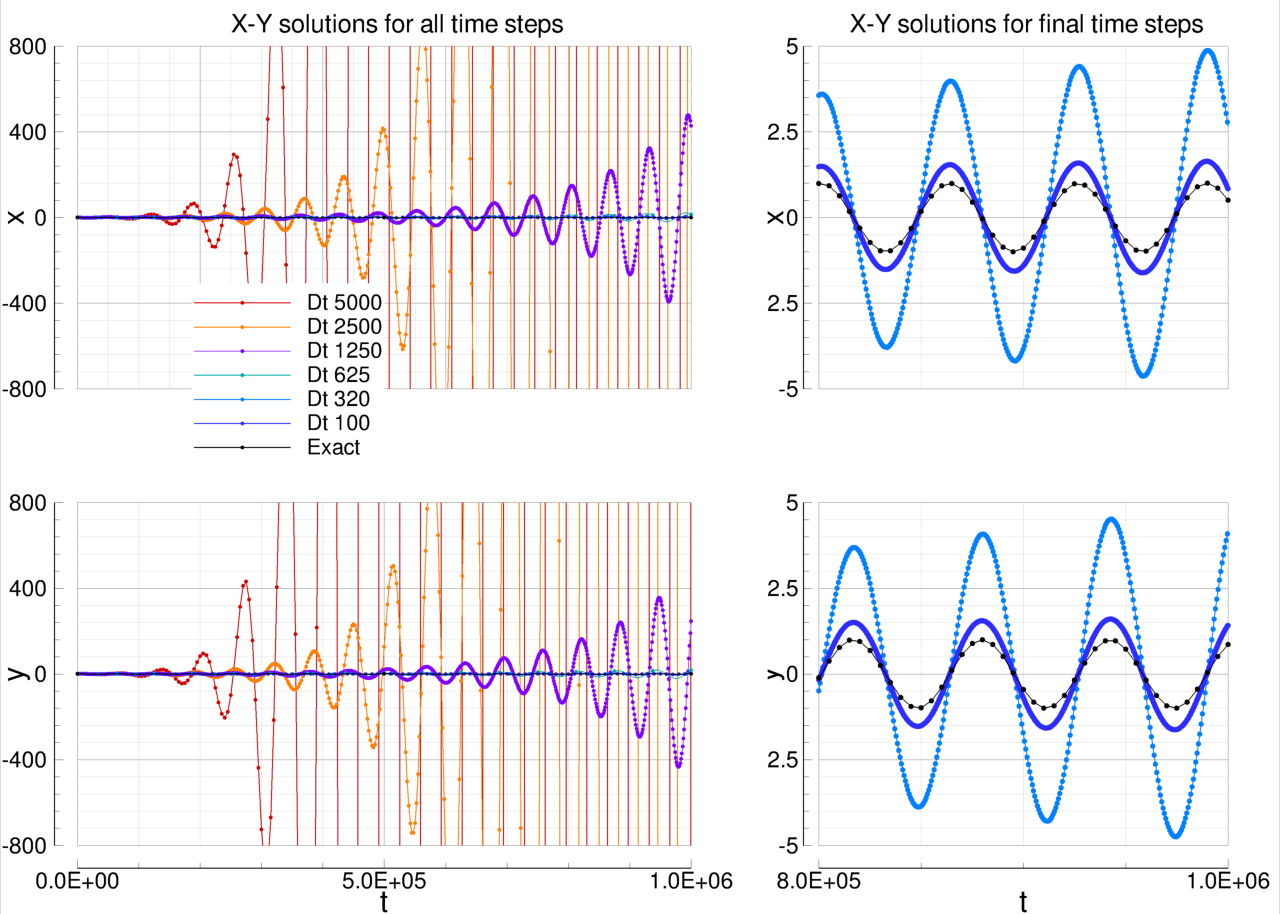
\includegraphics[width=1.00\textwidth]{errors-analysis/oscillation/errors_analysis-oscillation-tvd-runge-kutta-1.png}
    \caption{1 stage}\label{fig:results-oscillation-tvd-runge-kutta-1}
  \end{subfigure}\quad%
  \begin{subfigure}[b]{0.45\textwidth}
    \centering
    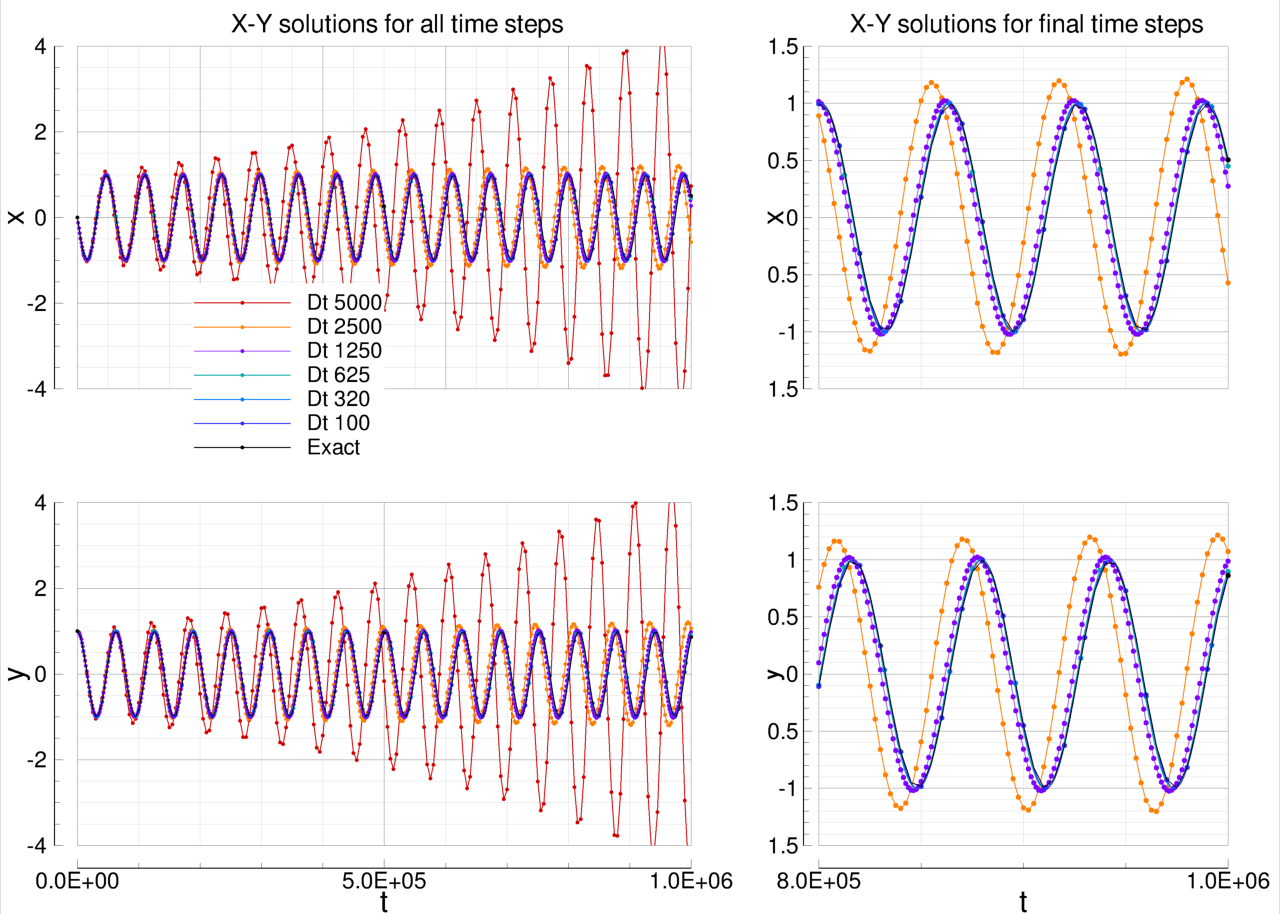
\includegraphics[width=1.00\textwidth]{errors-analysis/oscillation/errors_analysis-oscillation-tvd-runge-kutta-2.png}
    \caption{2 stages}\label{fig:results-oscillation-tvd-runge-kutta-2}
  \end{subfigure}\\
  \begin{subfigure}[b]{0.45\textwidth}
    \centering
    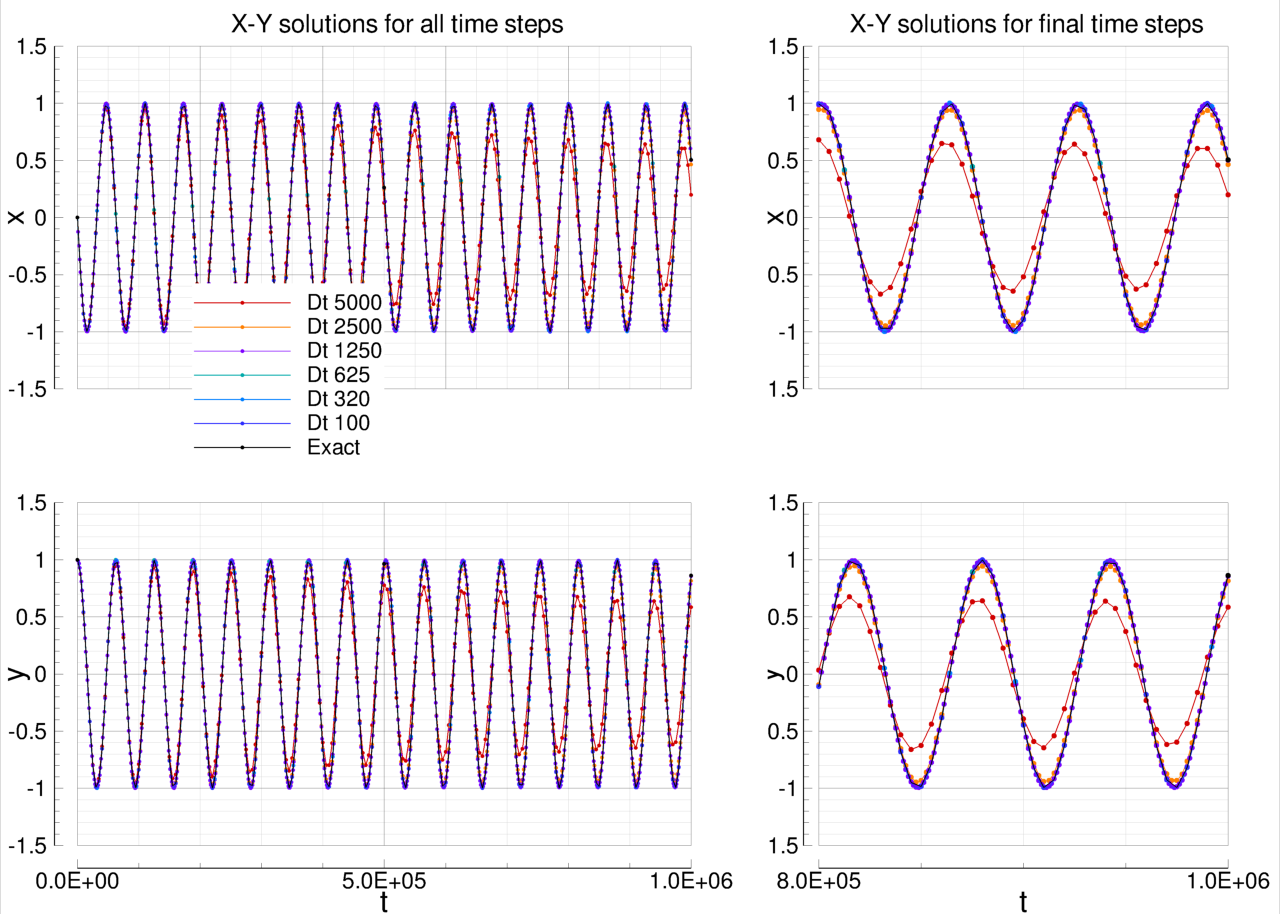
\includegraphics[width=1.00\textwidth]{errors-analysis/oscillation/errors_analysis-oscillation-tvd-runge-kutta-3.png}
    \caption{3 stages}\label{fig:results-oscillation-tvd-runge-kutta-3}
  \end{subfigure}\quad%
  \begin{subfigure}[b]{0.45\textwidth}
    \centering
    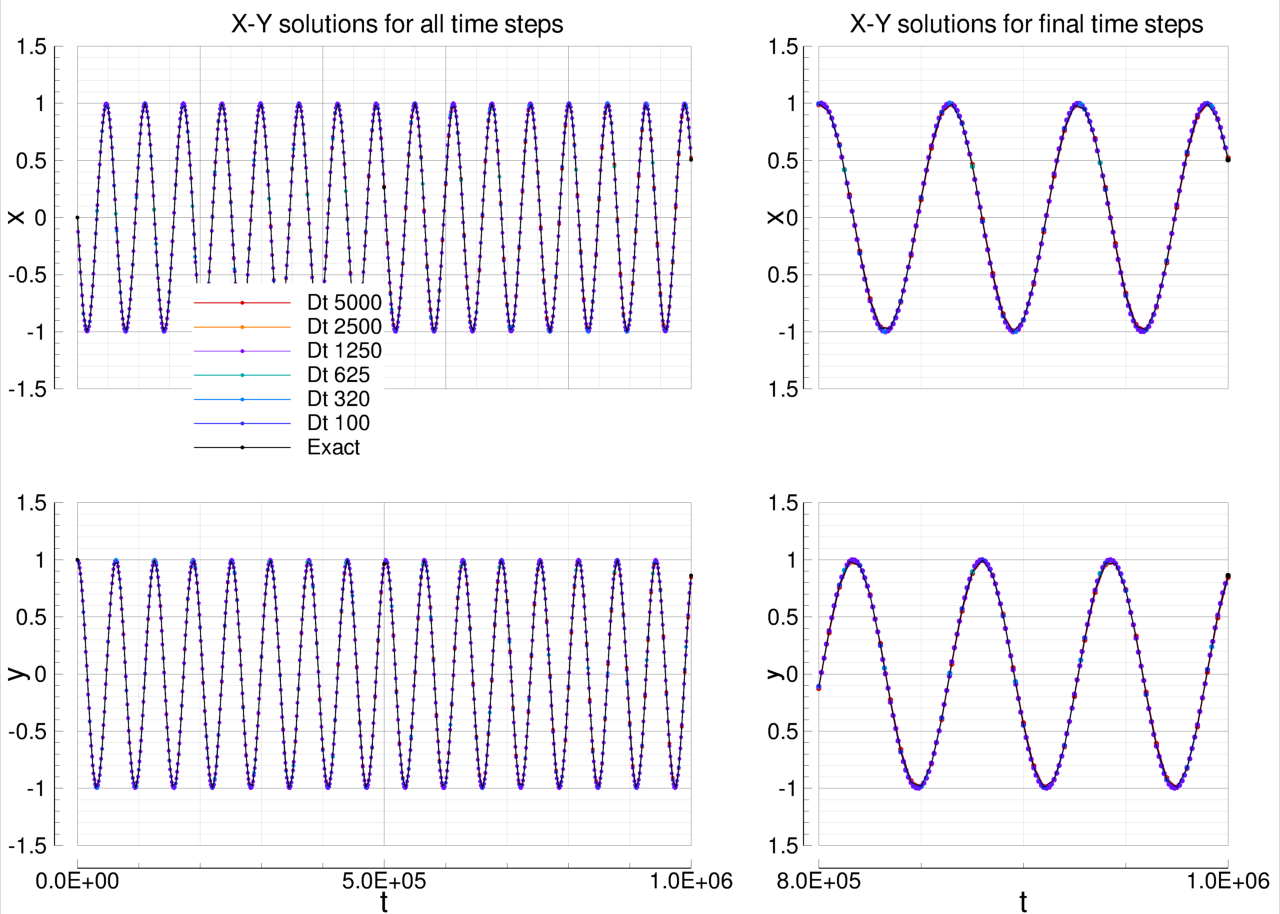
\includegraphics[width=1.00\textwidth]{errors-analysis/oscillation/errors_analysis-oscillation-tvd-runge-kutta-5.png}
    \caption{5 stages}\label{fig:results-oscillation-tvd-runge-kutta-5}
  \end{subfigure}\\
  \caption{Oscillation equations solutions computed by means of TVD/SSP Runge-Kutta solvers}\label{fig:results-oscillation-tvd-runge-kutta}
\end{figure}

